\chapter{Introduzione}

\section{Le basi del machine learning}

\subsubsection{Gli ingredienti del machine learning:}

\begin{itemize}
  \item [$\Rightarrow$] \fancyglitter{Task}: specifica di cosa si vuole fare;
  \item [$\Rightarrow$] \fancyglitter{Modelli}: il modello matematico per affrontare un determinato task;
  \item [$\Rightarrow$] \fancyglitter{Features}: il modo con cui sono descritti gli esempi.
\end{itemize}

\nt{L'\fancyglitter{apprendimento automatico} ruota attorno all'idea di estrarre una regola generale per risolvere un problema a partire da problemi già risolti.}

\ex{Etichettatura delle email spam}{
  \begin{center}
    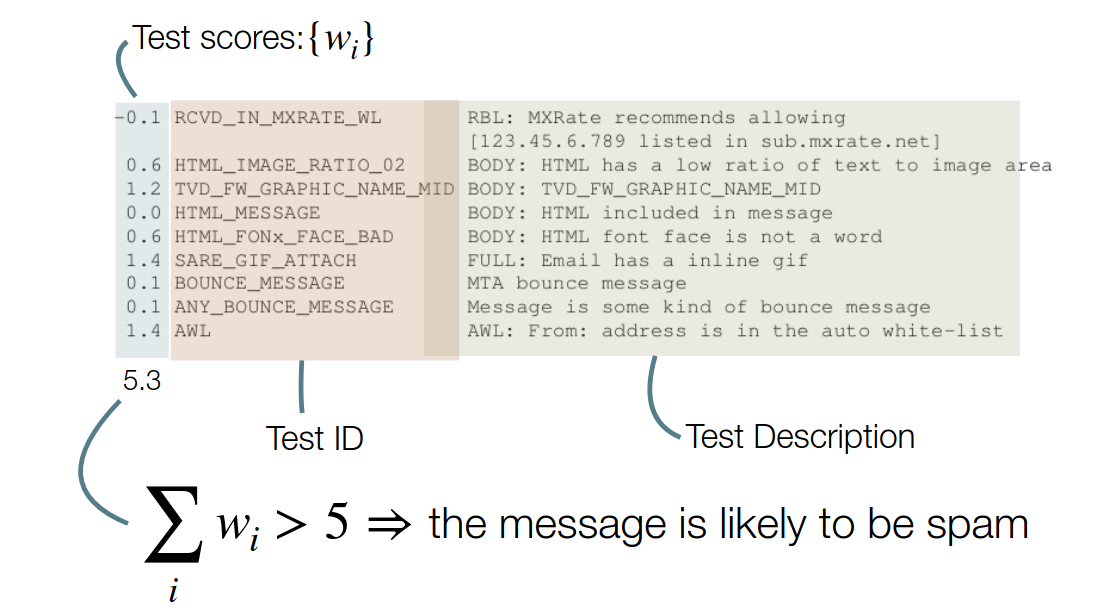
\includegraphics[scale=0.3]{01-Introduzione/Spam.png}
  \end{center}
  SpamAssassin è un filtro open-source usato per filtrare lo spam. Esso non lavora sul testo, ma su alcune \textit{feature} della mail. 
  \begin{center}
    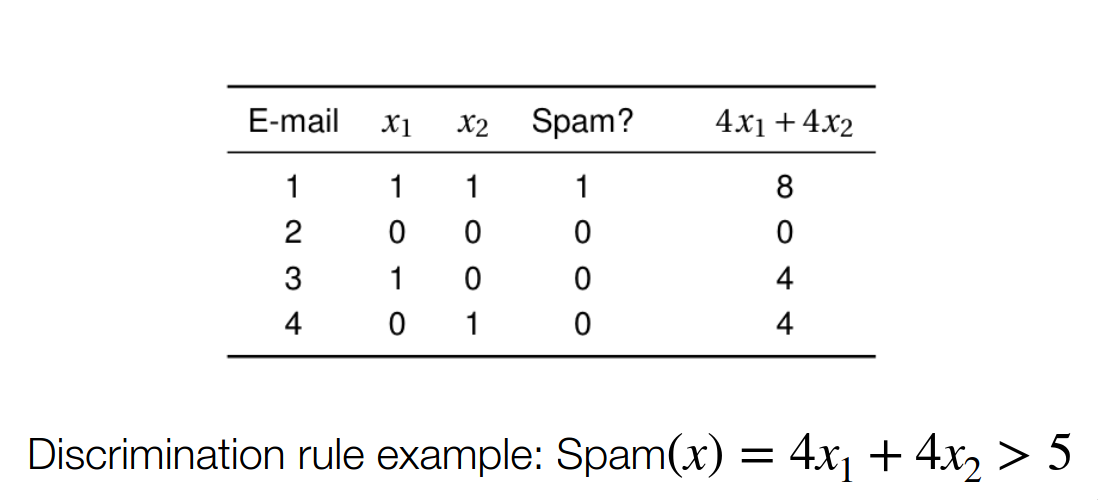
\includegraphics[scale=0.3]{01-Introduzione/Spam2.png}
  \end{center}
}

\dfn{Apprendimento automatico}{
  L'apprendimento automatico è lo studio sistematico di algoritmi e sistemi che migliorano le loro conoscenze e performance con l'esperienza.

  L'apprendimento automatico è interessato a usare le giuste features per costruire il giusto modello per ottenere buone performance sul giusto task.
}

\qs{}{
  L'apprendimento automatico come può aiutarci a risolvere un task?
}
\begin{figure}[h]
  \centering
  \begin{minipage}{0.45\textwidth}
    \centering
    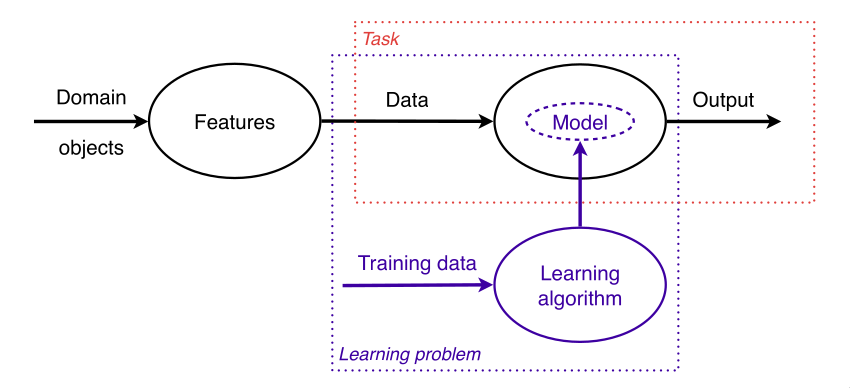
\includegraphics[scale=0.3]{01-Introduzione/ML.png}
  \end{minipage}\hfill
  \begin{minipage}{0.45\textwidth}
    \centering
    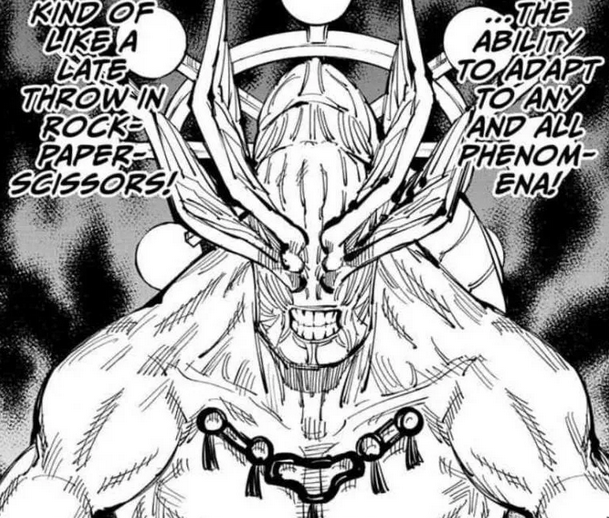
\includegraphics[scale=0.3]{01-Introduzione/Maho.png}
  \end{minipage}
\end{figure}

  \subsubsection{}
Dal dominio dell'applicazione arrivano degli oggetti descritti tramite features che vengono utilizzate per creare dei \fancyglitter{training data} e un \fancyglitter{dataset}. Questi vengono usati per costruire un modello per calcolare un output.

\nt{Per risolvere un task bisogna sfruttare un modello. Per risolvere un problema di apprendimento bisogna trovare un algoritmo di apprendimento.}

\subsection{Tasks}

\dfn{Tasks predittivi}{
  Un task predittivo è focalizzato sul predirre una variabile sulla base degli esempi. Si parte da problemi vecchi per trovare la soluzione a \newfancyglitter{nuovi} problemi.
}

\cor{Overfitting}{
  L'Overfitting è un adattamento eccessivo al dataset di allenamento per cui, messi di fronte a nuovi problemi, non si riesce a trovare una soluzione soddisfacente.
}

\subsubsection{I tasks predittivi possono essere:}

\begin{itemize}
  \item \fancyglitter{binari e multi-classe:} di categorizzazione;
  \item \fancyglitter{Regressivi:} con un target numerico;
  \item \fancyglitter{Clustering:} un target sconosciuto.
\end{itemize}

\nt{IL Clustering fa anche parte dei tasks descrittivi.}

\dfn{Tasks descrittivi}{
  Un task descrittivo si concentra sul fornire regolarità nel dataset.
}


  \begin{center}
    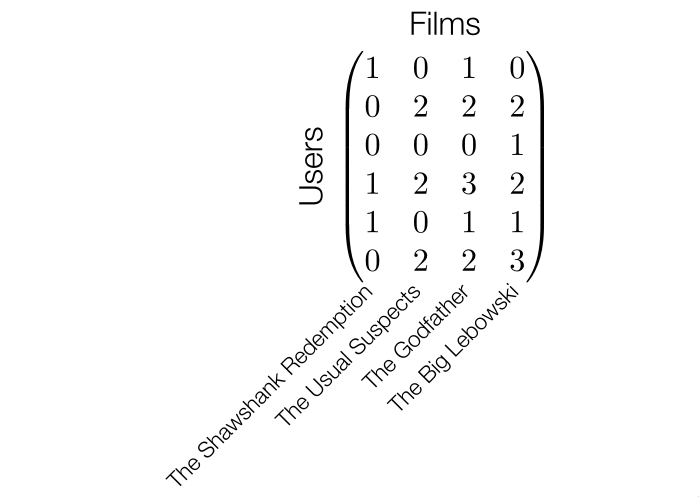
\includegraphics[scale=0.3]{01-Introduzione/M1.png}
  \end{center}

  \subsubsection{}
  Questa matrice rappresenta i voti dati da utenti a dei film. Si vogliono estrapolare le caratteristiche di questi film che hanno generato questi voti. Guardando questa matrice individualmente è difficile, per cui si compone con altre matrici.

  \begin{center} 
    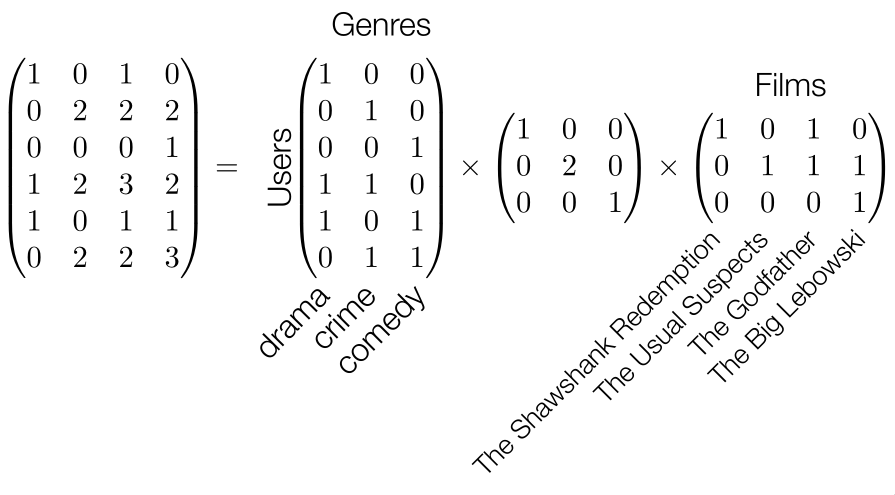
\includegraphics[scale=0.3]{01-Introduzione/M2.png}
  \end{center}

\subsection{Modelli}

\subsubsection{Ci sono 3 possibili tipi di modelli:}

\begin{itemize}
  \item \fancyglitter{Geometrici:} modelli che usano l'intuizione dalla geometria per risolvere il problema;
  \item \fancyglitter{Probabilistici:} usano il calcolo delle probabilità;
  \item \fancyglitter{Logici}.
\end{itemize}

\dfn{Modelli geometrici}{
  Nei modelli geometrici gli esempi sono punti di uno spazio vettoriale e la loro classificazione corrisponde a trovare un iperpiano che separi i punti positivi da quelli negativi.

}

\ex{Modello geometrico}{
  
  \begin{center} 
    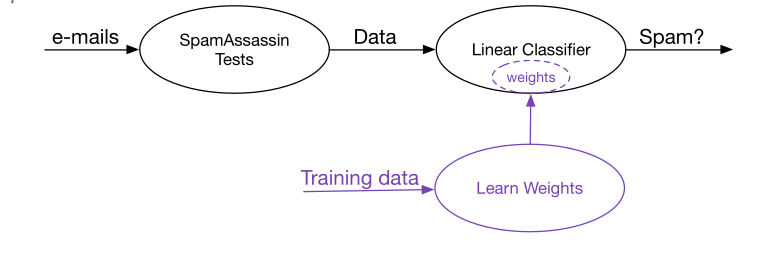
\includegraphics[scale=0.5]{01-Introduzione/Spam3.png}
  \end{center}
}

\dfn{Modelli probabilistici}{
Nei modelli probabilistici si fanno delle stime con dei classificatori probabilistici. Dopo di che si usano delle regole di decisione.

}

\ex{Modello probabilistico}{
  
  \begin{center} 
    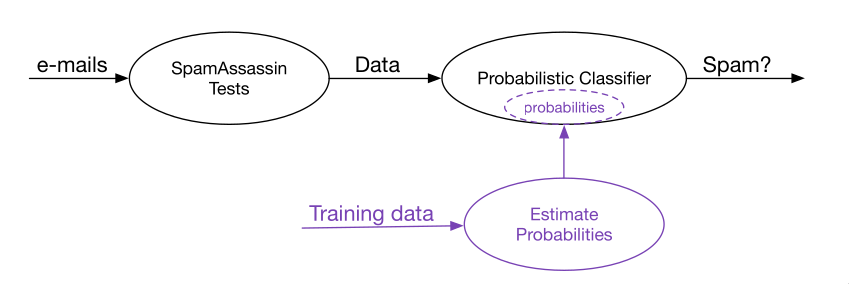
\includegraphics[scale=0.5]{01-Introduzione/Spam4.png}
  \end{center}
}

\nt{Uno degli algoritmi più semplici che si utilizza con i modelli probabilistici è l'assunzione di Naive Bayes. Si assume che x1 e x2 siano indipendenti tra loro per cui si possono calcolare solo i valori di x1 e di x2 individualmente.}



\dfn{Modelli logici}{
 Nei modelli logici si utilizza la logica. Si hanno una serie di regole.
}

\ex{Modello logico}{
  
  \begin{center} 
    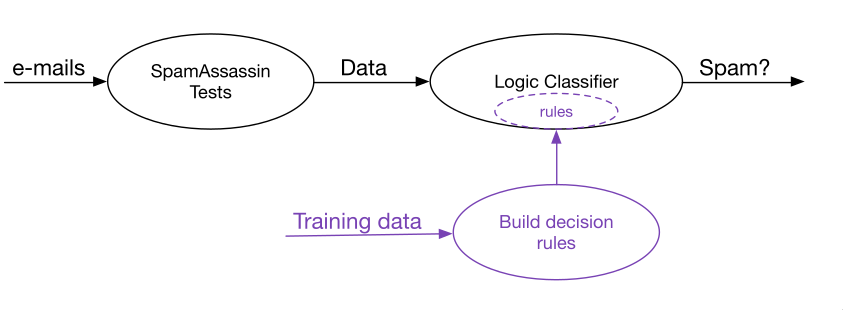
\includegraphics[scale=0.5]{01-Introduzione/Spam5.png}
  \end{center}
}

\subsection{Features}

\dfn{Features}{
  Il modo in cui si descrivono i propri dati. Possono facilitare il lavoro di apprendimento se correttamente usate.
}

\ex{Coseno}{
    
  \begin{center} 
    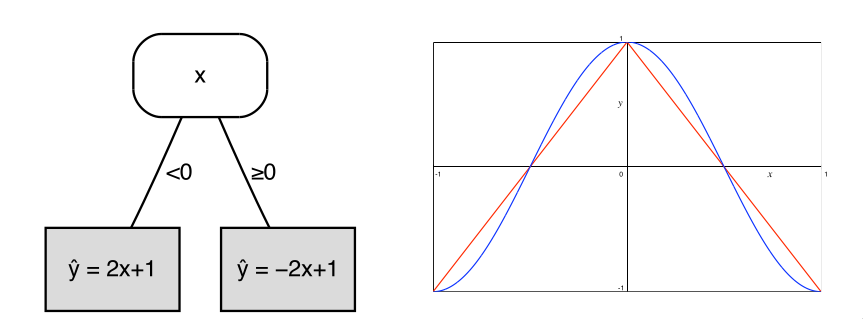
\includegraphics[scale=0.5]{01-Introduzione/COS.png}
  \end{center}

  Due rappresentazioni della funzione coseno: a destra si utilizza una variabile di regressione, a destra un'approssimazione lineare.
}

\section{Tasks}

\subsubsection{I task più comuni sono:}

\begin{itemize}
  \item \fancyglitter{classificazione};
  \item \fancyglitter{Punteggio e classifica};
  \item \fancyglitter{Stima probabilistica};
  \item \fancyglitter{Regressione}.
\end{itemize}

\subsection{classificazione}

\dfn{classificazione}{
  La classificazione è il task in cui si ha come obiettivo la costruzione di un modello \^c: $\bbX \to \bbC$ in cui $\bbC = \{C_1, C_2, ..., C_k\}$. Questo modello è un'approssimazione
   del mondo reale. 

   Un esempio è una coppia $(x, c(x)) \in \bbX x \bbC$.  
}

\clm{Il problema dell'induzione}{}{
  L'induzione partendo dai dati di un dataset è generalmente infondata senza ulteriori informazioni.
}

\nt{Il mondo non è semplice, per cui il rasoio di Occame non sempre funziona. Spesso però si utilizzano preconcetti e bias induttivi per avere apprendimento automatico.}

\dfn{classificazione binaria}{
  La classificazione binaria è il caso in cui si hanno solo 2 opzioni (spesso 0 e 1).
}

\nt{Dalla classificazione binaria si può passare alla classificazione multi-classe senza sviluppare nuovi algoritmi.}

  
  \begin{center} 
    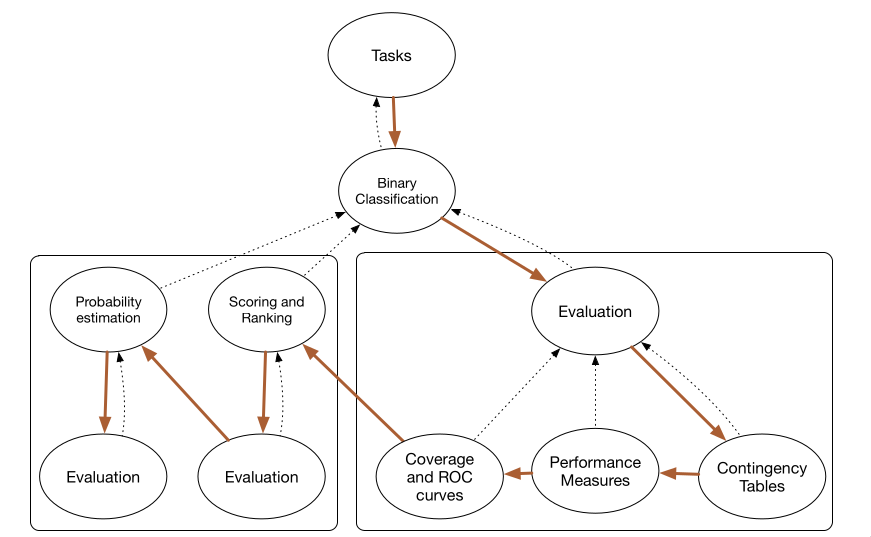
\includegraphics[scale=0.5]{01-Introduzione/Graph.png}
  \end{center}

\dfn{Alberi di decisione}{
  Alberi per visualizzare i dati. Ogni nodo corrisponde a una features.
}

\dfn{Alberi di Features}{
  Alberi per visualizzare i dati. Si ha una suddivisione dei vari esempi divisi per etichette.
}


\begin{center} 
 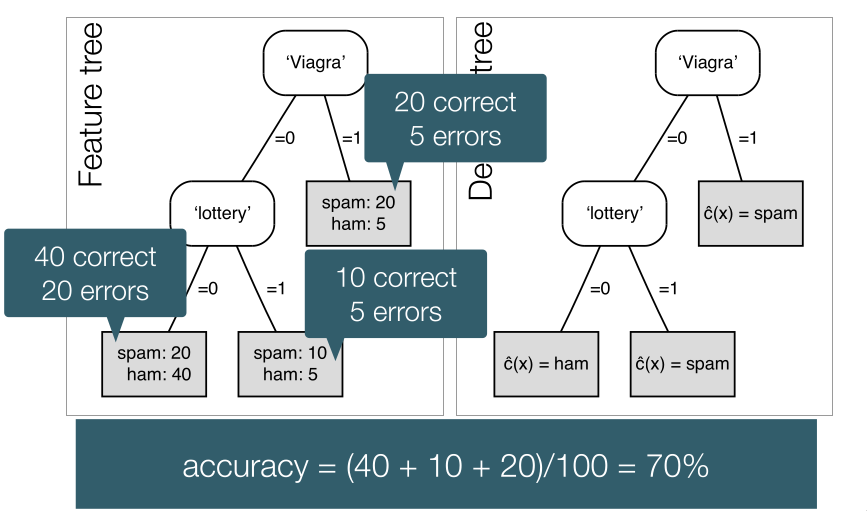
\includegraphics[scale=0.5]{01-Introduzione/AD.png}
\end{center}

\dfn{Tavola di contingenza}{
  Tavola in cui le colonne corrispondono alle predizioni e le righe al mondo reale. Nella loro intersezione si ha il numero di esempi predetti in un certo modo e hanno una certa etichetta (TP, TN, FT, FN).
}


\begin{center} 
 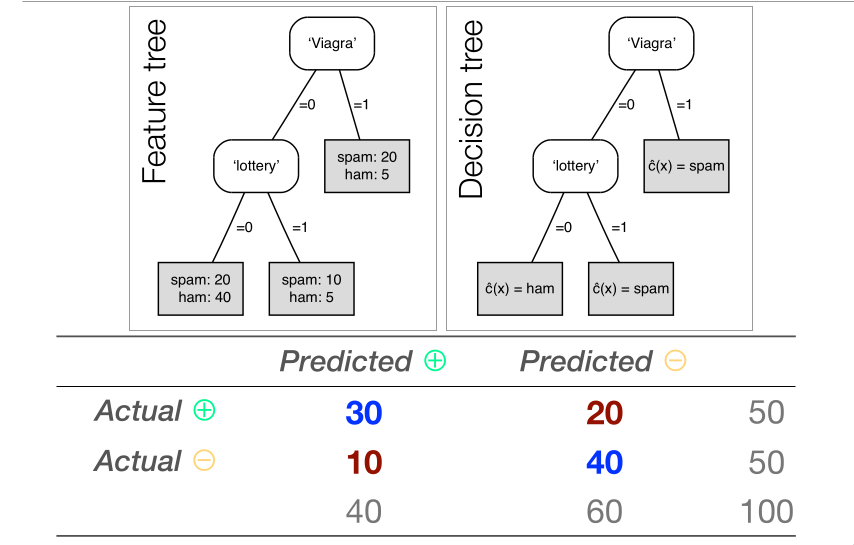
\includegraphics[scale=0.5]{01-Introduzione/TC.png}
\end{center}

\dfn{Grafico di copertura}{
  Grafico per visualizzare le informazioni della tavola di contingenza.
}


\begin{center} 
 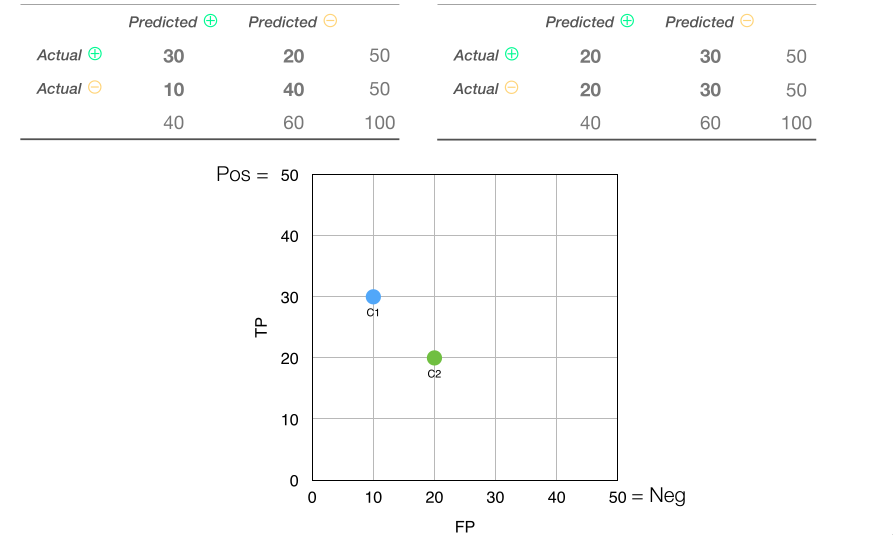
\includegraphics[scale=0.5]{01-Introduzione/GC.png}
\end{center}

\nt{I classificatori che si trovano sulla bisettrice del piano cartesiano sono imprevedibili e quindi poco interessanti. Più un classificatore ha la coordinata x bassa e y alta più è preciso.}

\begin{figure}[h]
  \centering
  \begin{minipage}{0.45\textwidth}
    \centering
    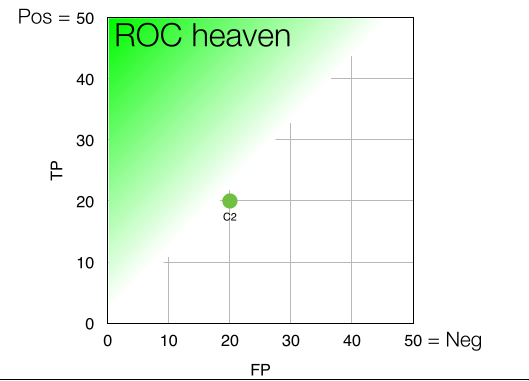
\includegraphics[scale=0.47]{01-Introduzione/ROCHEAVEN.png}
  \end{minipage}\hfill
  \begin{minipage}{0.45\textwidth}
    \centering
    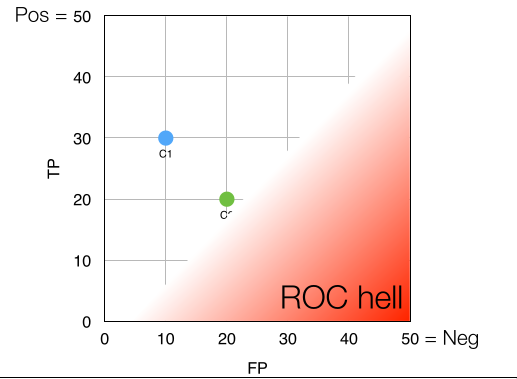
\includegraphics[scale=0.47]{01-Introduzione/ROCHELL.png}
  \end{minipage}
\end{figure}

\nt{Tutti i classificatori che stanno su una retta con pendenza 1 hanno la stessa \fancyglitter{accuratezza}.}

\dfn{Avg recall}{
  \newfancyglitter{avg recall} = (recall + specificity) / 2 = (TP/POS + TN/NEG)/2

  Se due classificatori hanno la stessa avg recall allora sono su linee parallele alla diagonale principale.
}

\begin{center} 
 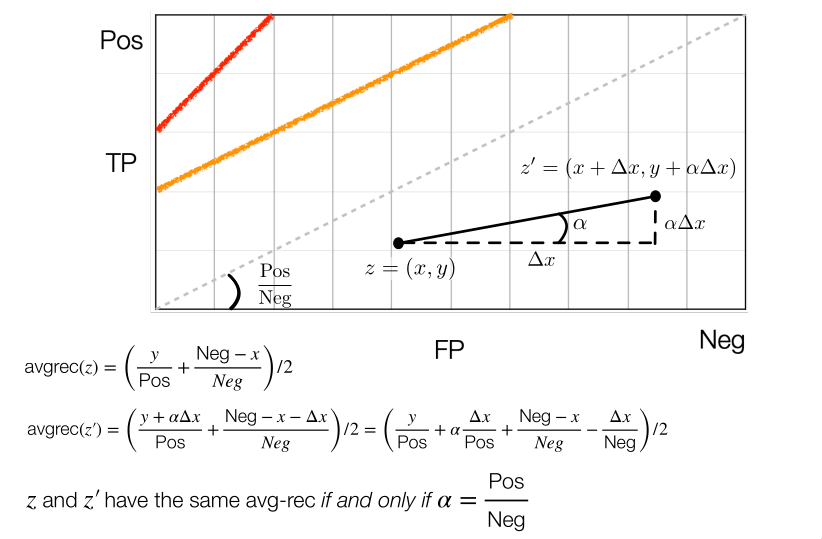
\includegraphics[scale=0.5]{01-Introduzione/avg.png}
\end{center}

\subsubsection{Roc Plots Properties}

Se si vogliono confrontare le performance di un classificatore su un dataset o su un altro si deve \fancyglitter{normalizzare} gli assi dividendo l'asse x per il numro di esempi negativi e l'asse y per il numero di esempi positivi. Così facendo si otterrà un quadrato con gli assi compresi tra 0 e 1.

\begin{center} 
 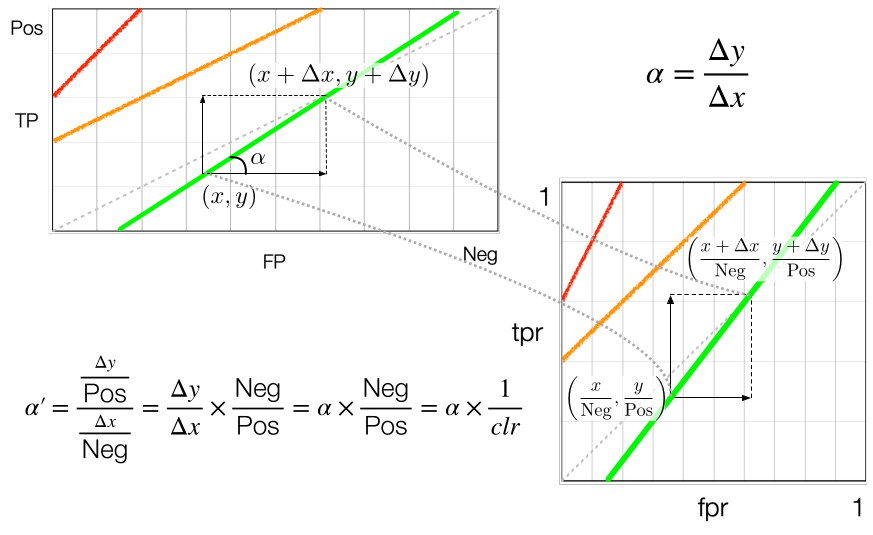
\includegraphics[scale=0.5]{01-Introduzione/Trasl.png}
\end{center}

\nt{Il clr è il class ratio.}

\subsubsection{Più di un Classificatore per una Singola Feature.}

\begin{center} 
 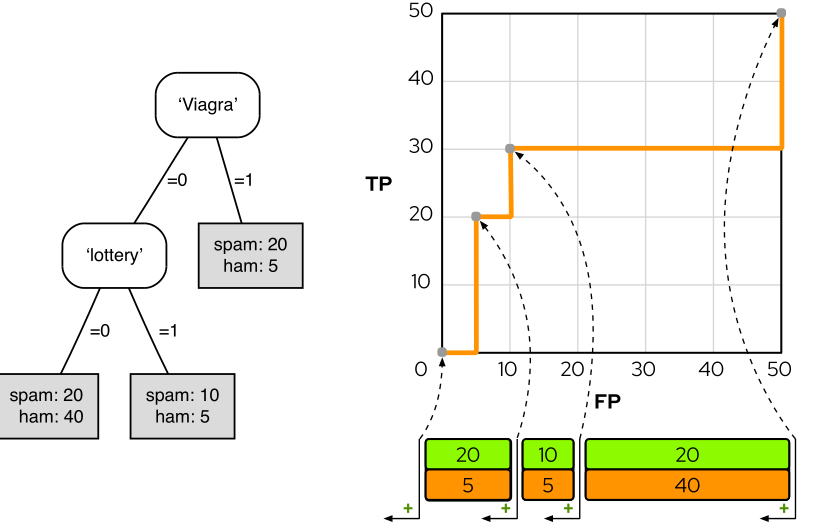
\includegraphics[scale=0.53]{01-Introduzione/MDT.png}
\end{center}

\qs{}{Come si considera il caso in cui il costo per FP (falsi positivi) e FN (falsi negativi) sono differenti?}

\begin{center} 
 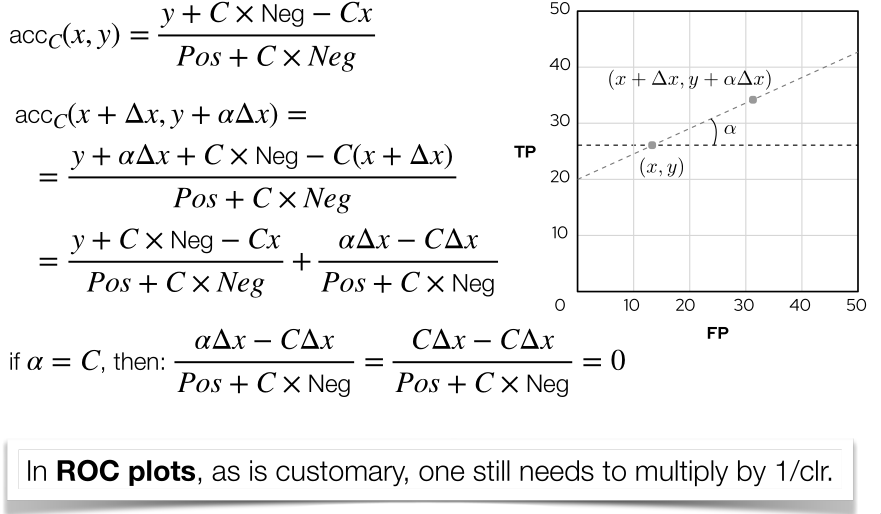
\includegraphics[scale=0.53]{01-Introduzione/FPFN.png}
\end{center}

\subsection{Scoring e ranking}

\dfn{Scoring classifier}{
  Uno scoring classifier è una mappatura \^s: $\bbX \to \bbR^k$ il cui output è un vettore (\^s (x) = \^s1(x),...,\^si(x)) dove i-esimo componente è lo score assegnato alla classe Ci per l'istanza x.
}

\nt{Se si hanno solo due classi si può considerare solo uno score. Gli score vanno interpretati nel contesto di un classificatore, sono misure della confidenza in una determinata predizione.}

\begin{center} 
 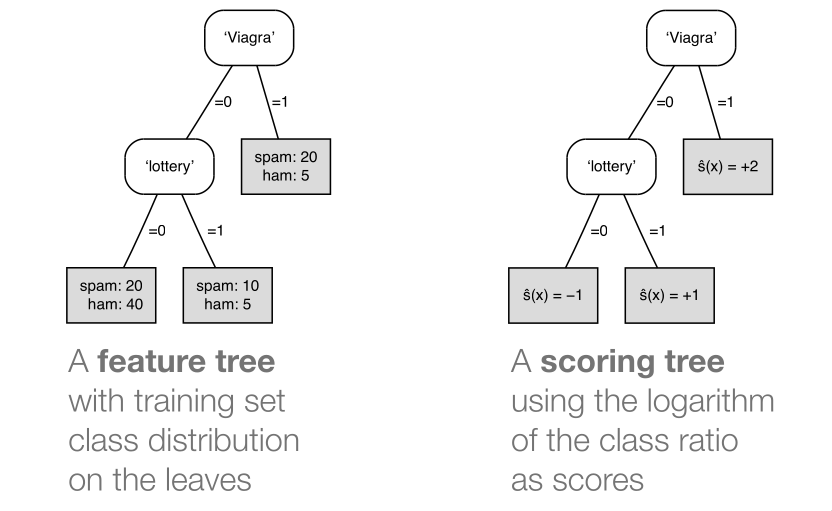
\includegraphics[scale=0.5]{01-Introduzione/ST.png}
\end{center}

\dfn{Margine}{
  Il margine assegnato dallo scoring classifier è positivo se \^s è corretto, negativo altrimenti. Il margine è il prodotto tra la classe dell'esempio e lo score.

  $$z(x) = c(x)\text{\^s}(x) =  \begin{cases}
  z(x) > 0 & \text{se la classificazione è corretta (cioè, } c(x) \text{ corrisponde alla classe prevista)} \\
  z(x) < 0 & \text{se la classificazione è incorretta (cioè, } c(x) \text{ non corrisponde alla classe prevista)} \\
  z(x) = 0 & \text{se lo score è esattamente al confine di decisione}
  \end{cases}$$

}


\subsubsection{Loss Function}

\dfn{Loss Function}{
  La funzione di loss cerca di pesare l'impatto degli esempi negativi. In 0 la funzione di loss vale 1, tende a infinito con margini molto piccoli (molto negativi).
  \[
  L: \mathbb{R} \to [0, \infty)
  \]
}

\nt{Le loss function sono importanti durante l'apprendimento perché sono usate per guidare la ricerca della soluzione ottimale. }

\subsubsection{Tipi di loss}

\cor{0-1 loss}{
  Si perde un'unità se si sbaglia e non si perde nulla se si indovina.
}

\begin{center} 
 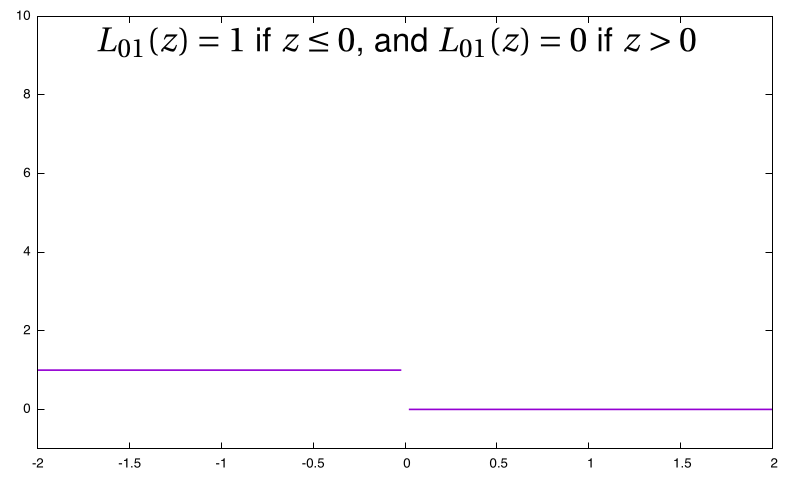
\includegraphics[scale=0.53]{01-Introduzione/01Loss.png}
\end{center}

\cor{Hinge loss}{
  La Hinge loss è una loss che è lineare per valori minori di 1 e vale 0 per valori maggiori di 1.
}

\begin{center} 
 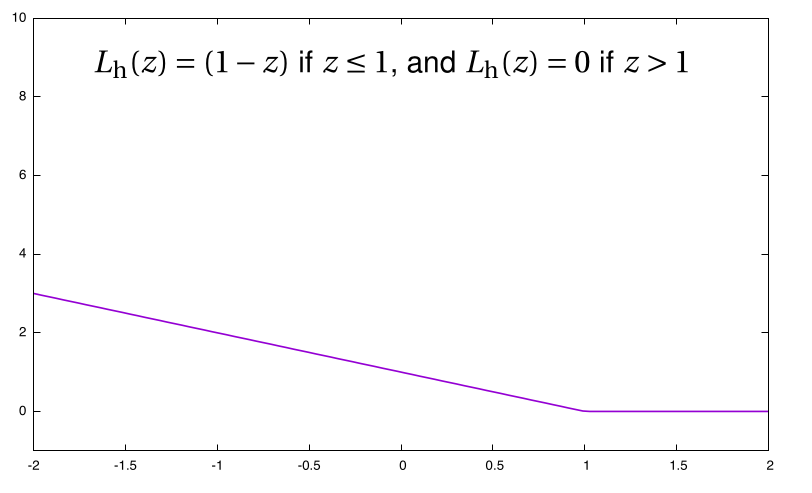
\includegraphics[scale=0.53]{01-Introduzione/Hinge loss.png}
\end{center}

\cor{Logistic loss}{Approssimazione continua della Hinge loss.}

\begin{center} 
 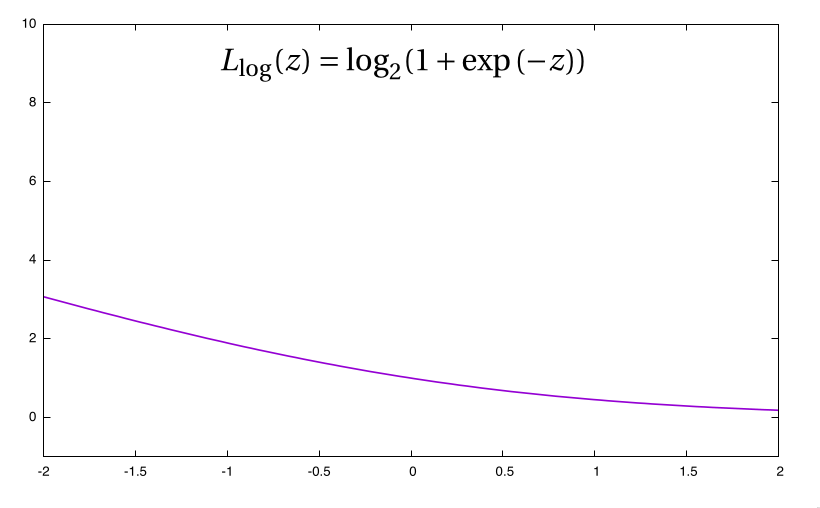
\includegraphics[scale=0.53]{01-Introduzione/Logistic loss.png}
\end{center}

\cor{Loss esponenziale}{Cresce rapidamente quando si stanno facendo errori.}

\begin{center} 
 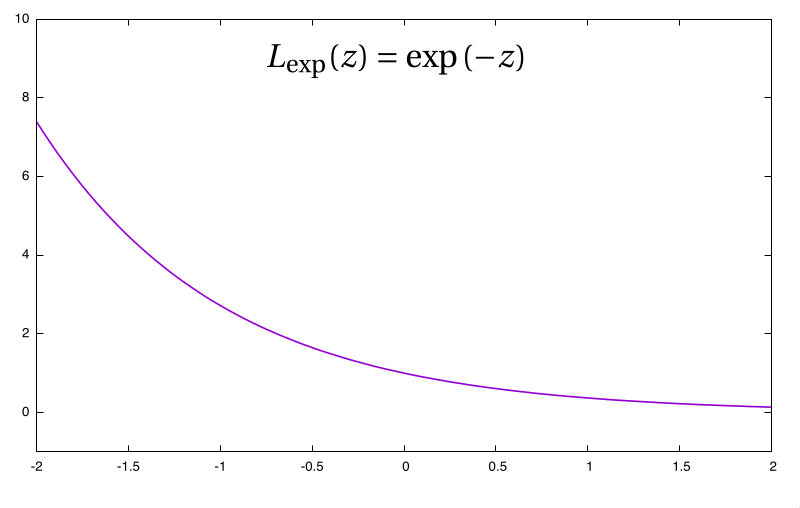
\includegraphics[scale=0.53]{01-Introduzione/Exp Loss.png}
\end{center}

\cor{Loss quadratica}{Se viene ottimizzata troppo si hanno modelli incogniti, funziona meglio con la regressione.}

\begin{center} 
 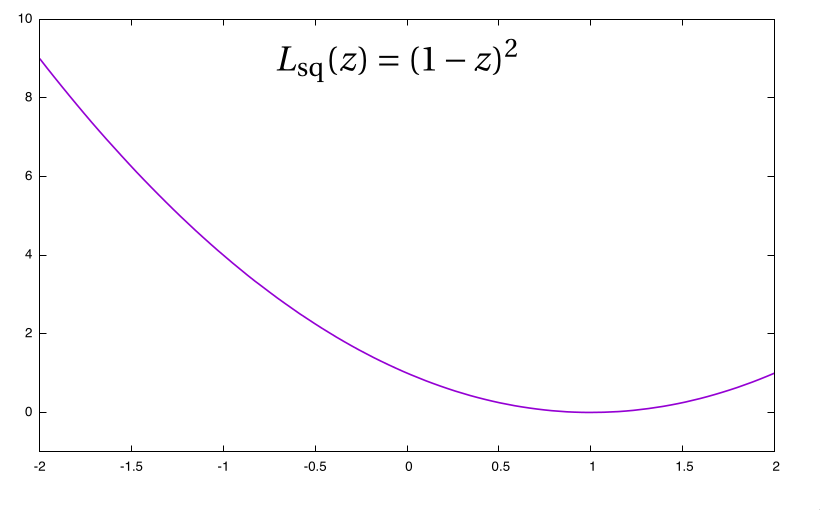
\includegraphics[scale=0.53]{01-Introduzione/Quad loss.png}
\end{center}

\subsubsection{Ranking}

\dfn{Ranking}{Ordina sulla base di uno score. Dall'esempio che è di classe più positiva a quello di classe meno positiva.}

\cor{Ranking Error Rate}{
\begin{center} 
 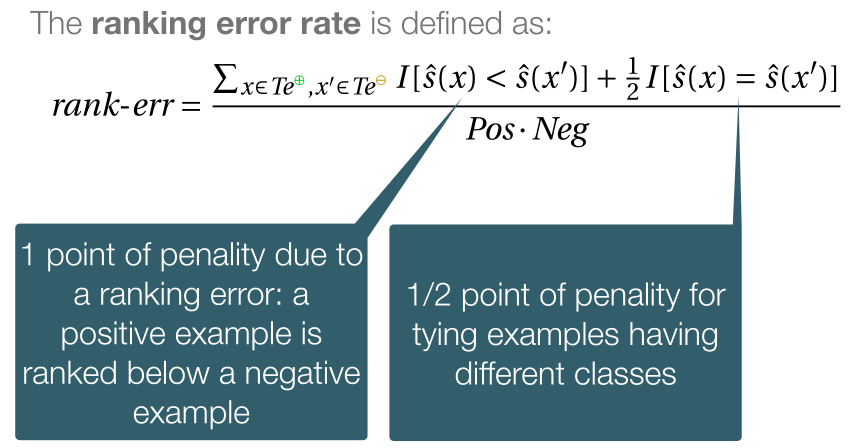
\includegraphics[scale=0.53]{01-Introduzione/Rank.png}
\end{center}
}

\ex{Ranking Error Rate}{
\begin{center} 
 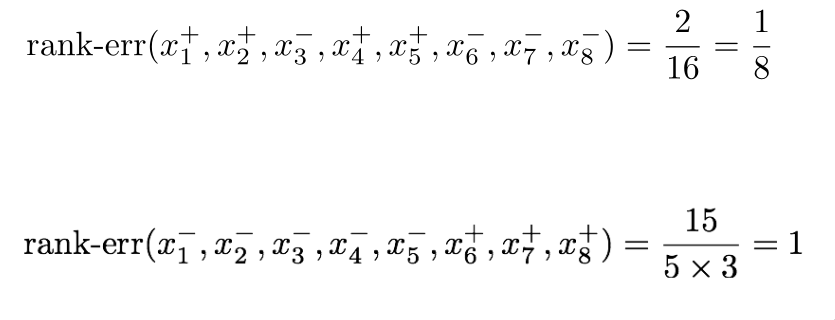
\includegraphics[scale=0.53]{01-Introduzione/Rank1.png}
\end{center}

}

\ex{Spam}{
  \begin{center} 
 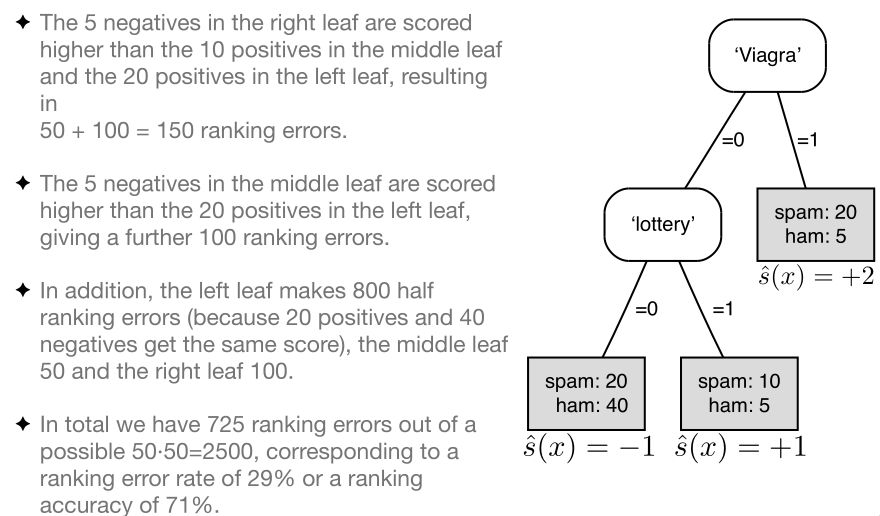
\includegraphics[scale=0.53]{01-Introduzione/Spam6.png}
\end{center}

}

\subsection{Stima Probabilistica}

\dfn{Stimatore probabilistico di classi}{
  Uno stimatore probabilistico di classi è un classificatore di scoring il cui output è un vettore di probabilità. 

  \[
    \hat{p}: \bbX \to [0, 1]^k
  \]

Scriviamo:

\[
  \hat{p}(x) = (\hat{p}_1(x),\dots,\hat{p}_k(x))
\]

dove l'i-esimo componente è la probabilità assegnata alla classe $C_i$ e $\displaystyle\sum_{i=1}^{k}\hat{p}_i(x) = 1$
}

\nt{Se si hanno solo 2 classi allora \^p(x) denota la probabilità stimata per le classi positive.}

  \begin{center} 
    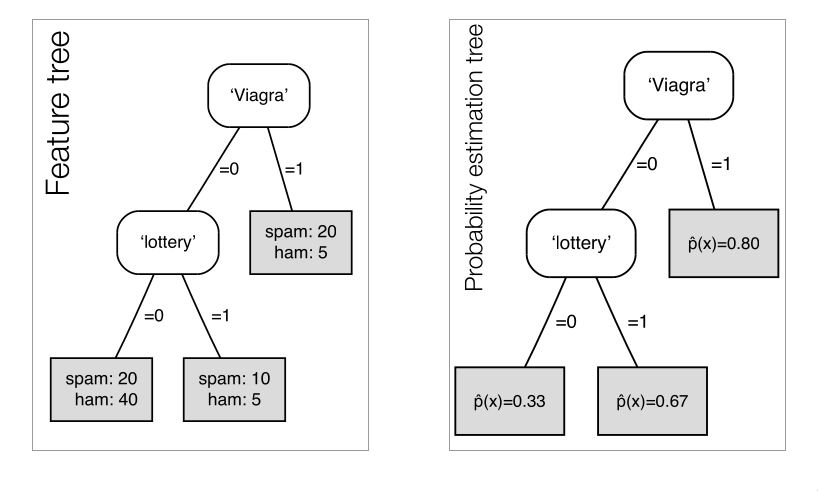
\includegraphics[scale=0.53]{01-Introduzione/prob.png}
\end{center}

\cor{Squared Error}{
    \begin{center} 
 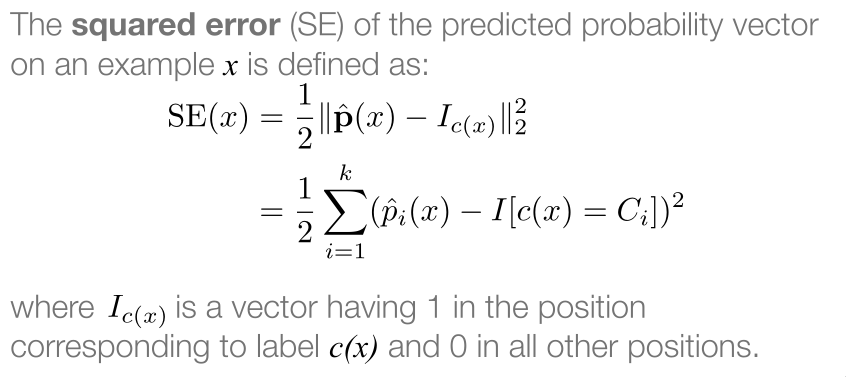
\includegraphics[scale=0.4]{01-Introduzione/SE.png}
\end{center}
}

\cor{Mean Squared Error}{
 Il mean squared error è la media aritmetica degli squared error.
}

\dfn{Probabilità Empiriche}{
  Le probabilità empiriche consentono di ottenere probabilità stimate da classificatori o rankers. Se si ha un insieme S di esempi etichettati e il numero di esempi in S di classe $C_i$ è scritto $n_i$ il vettore di probabilità empiriche associato ad S sarà:

  \[
    \hat{p}(S) = (n_1/|S|,\dots, n_k/|S|)
  \]
}

\cor{Correzione di Laplace}{
  Se si ha un insieme S e dentro si hanno $n_i$ elementi di classe $C_i$ per ogni classe si fa finta di avere un esempio aggiuntivo.

  \[
    \hat{p}_i(S) = \frac{n_i + 1}{|S| + k}
  \]

Si può applicare anche:

  \[
    \hat{p}_i(S) = \frac{n_i + m*\pi_i}{|S| + m}
  \]
La Correzione di Laplace è un caso speciale in cui $m = k$ e la distribuzione è uniforme ($\pi_i = \frac{1}{k}$)
}

\subsection{Oltre la Classificazione Binaria}

    \begin{center} 
 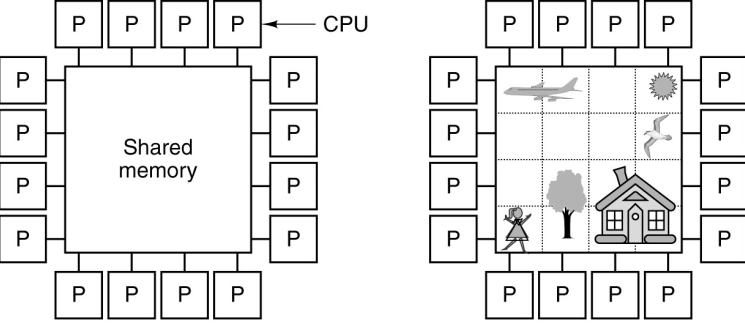
\includegraphics[scale=0.42]{01-Introduzione/Multi.png}
\end{center}

\subsubsection{Schemi per estendere la classificazione binaria al caso multi-classe:}


\begin{itemize}
  \item one-vs-rest:
    \begin{itemize}
      \item apprendimento non ordinato;
      \item apprendimento in ordine fisso.
    \end{itemize}
  \item one-vs-one:
    \begin{itemize}
      \item simmetrici;
      \item asimmetrici.
    \end{itemize}
\end{itemize}

\subsubsection{One-vs-Rest (non ordinato)}

\begin{center} 
 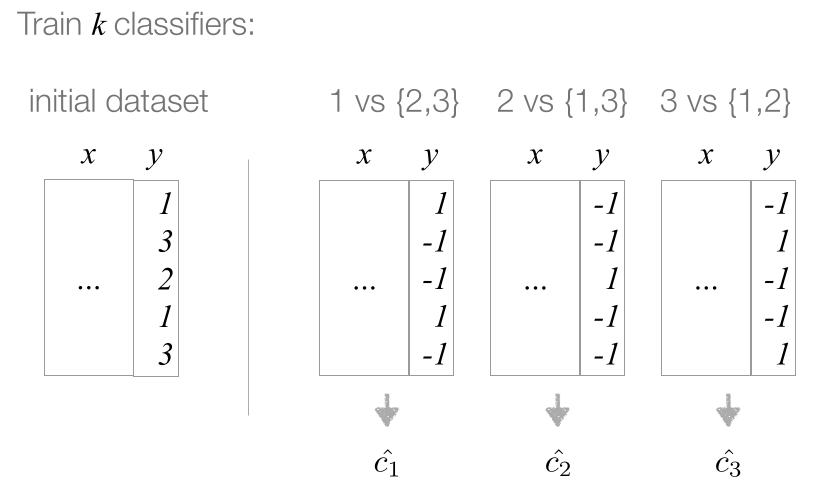
\includegraphics[scale=0.5]{01-Introduzione/ovro.png}
\end{center}

\nt{Si può costruire una matrice con il codice di output: in ogni riga si mette una classe, in ogni colonna si mette un classificatore che si vuole costruire e in ogni cella il valore che si vuole in output.}

\begin{center} 
 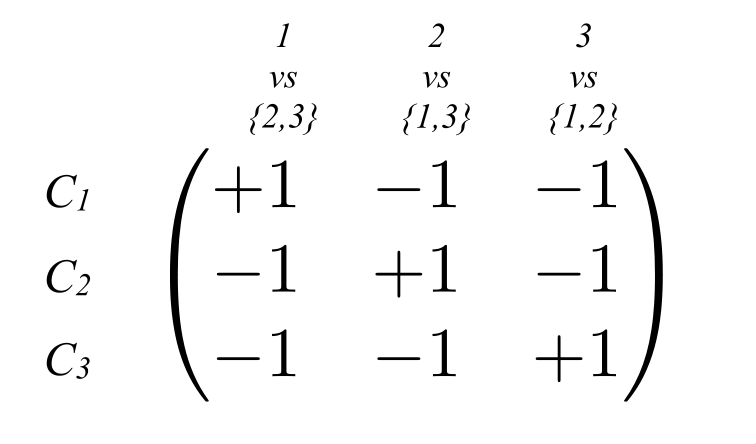
\includegraphics[scale=0.35]{01-Introduzione/ovro1.png}
\end{center}

\subsubsection{One-vs-Rest (ordinato)}

\begin{center} 
 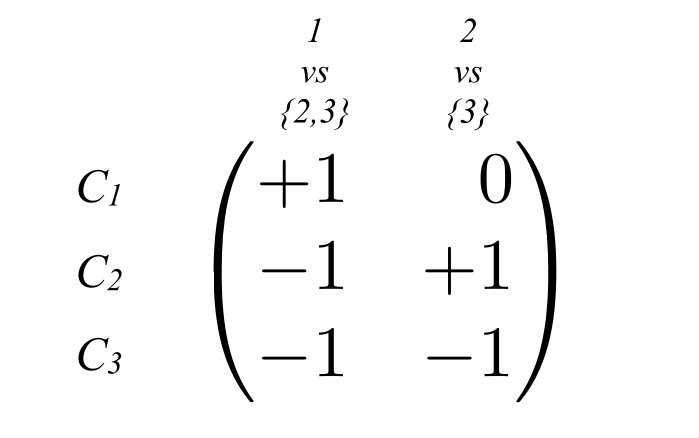
\includegraphics[scale=0.35]{01-Introduzione/ovro2.png}
\end{center}

\subsubsection{One-vs-one (simmetrico)}

\begin{center} 
 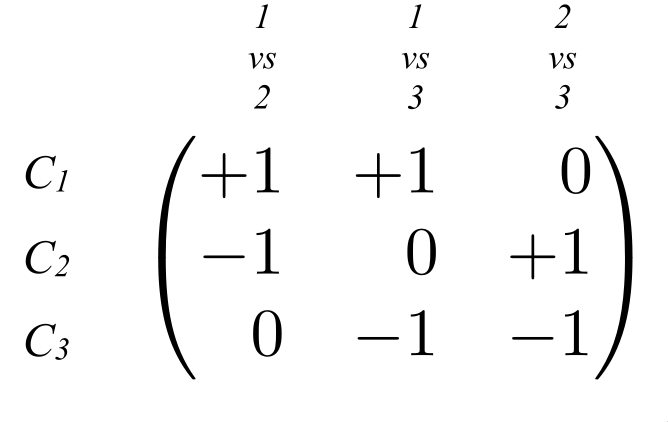
\includegraphics[scale=0.35]{01-Introduzione/ovos.png}
\end{center}

\subsubsection{One-vs-one (asimmetrico)}

\begin{center} 
 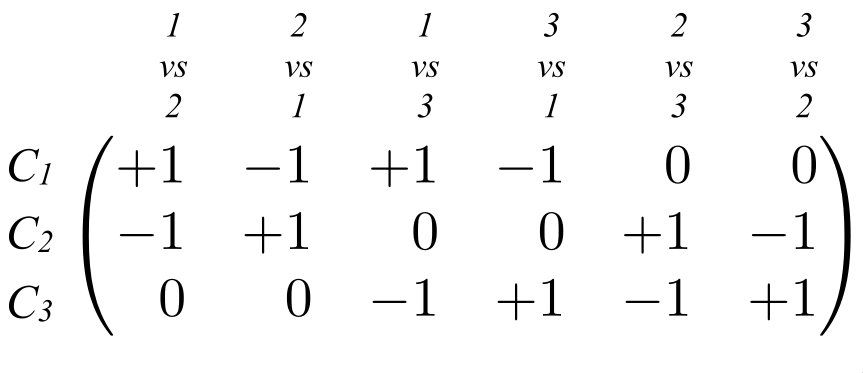
\includegraphics[scale=0.35]{01-Introduzione/ovoa.png}
\end{center}

\nt{Per classificare un nuovo esempio (vettore) si cerca la riga più simile.}

\clm{Difficoltà nell'applicare one-vs-rest e one-vs-one}{}{

  \begin{itemize}
    \item   Nel caso one-vs-rest il singolo classificatore vede un dataset molto sbilanciato sebbene il dataset di partenza fosse bilanciato. 
    \item Nel caso one-vs-one il problema è mitigato assegnando 0 agli esempi che non appartengono alle due etichette scelte. Però è problematico quando si ha scarsità nei dati. 
  \end{itemize}
}

\qs{}{Come si rompono i pareggi?}

\begin{enumerate}
  \item Si aggiungono classificatori;
  \item Se si ha un algoritmo di apprendimento in grado di assegnare uno score si può scegliere il valore su cui si è più confidenti.
\end{enumerate}








